\chapter{Conception et développement de l'application}
 \minitoc
 \section{Généralités}
 Le développement de l'application s'est fait principalement à partir du langage Python et du framework Flask que nous avons rencontré durant cette année scolaire dans le cadre de la WebBD et du TAPS. Le module développé présente donc deux parties: 
 \begin{itemize}
         \item La partie Front-end, c'est à dire la partie client qui permet au client d'appliquer des fonctionnalités CRUD à la base de données à partir de méthodes FORM
         \item La partie Back-end, c'est à dire la partie serveur qui gère ces modifications dans la base de données
      \end{itemize}
      Un schéma résumant l'ensemble des interactions serveur/client sera fourni à la fin de ce chapitre.\\
      
     On utilise dans cette partie un nombre de librairies Python pour parvenir à nos fins:\\
     -Flask qui permet d'utiliser le framework Flask \\
     -pdfkit qui premet de convertir des urls en pdf\\
     -sqlite3 qui permet d'accéder et de modifier la base de données en utilisant le langage SQL\\
 \section{Partie Front-end de l'application}
 La problématique du sujet nous demandais de créer une application permettant à l'utilisateur d'effectuer des requêtes (SQL ou autres) qui interagissent avec la base de données et d'en conserver le résultat sous forme HTML ou PDF.
 \subsection{Présentation de l'interface utilisateur}
 Les requêtes des utilisateurs varient grandement selon l'identité de l'utilisateur, en effet, on peut classer les profils utilisateurs dans quatre grandes catégories compte tenue de la nature des données:
\begin{itemize}
         \item Élèves qui seront intéressés uniquement par leur profil candidat
         \item Professeurs qui seront intéressés par les étudiants de leur établissement
         \item Administrateurs qui savent utiliser le SQL et veulent uploader des fichiers .xlsx ou .csv pour mettre à jour les données
         \item Curieux qui veulent tout simplement connaître des informations plus générales sur l'ensemble du concours de l'institut Mines-Télécom.
      \end{itemize}
L'objectif ici étant de permettre à tout le monde d'accéder à l'ensemble des données qui leur sont pertinentes le plus rapidement possible.
De cette manière,un utilisateur non-identifié doit alors déclarer son identité sur la page principale de l'application. Une fois identifié il se retrouvera sur une page de connexion ( à l'exception du profil "Curieux"), qui permettra à l'application de confirmer son identité en comparant les informations fournies avec celles données par la partie serveur de l'application.

FIGURE
\subsubsection{Interface Élève}
L'utilisateur "Élève" qui est identifié par son code candidat (unique) et son nom. Une fois, la connexion établie, il arrivera à sa page personnelle où il aura accès à plusieurs information:\\

\begin{itemize}
         \item Les informations personnelles le concernant tirés de la table candidat, modifiable
         \item Les notes obtenues aux écrits et aux oraux (si ces derniers ont eu lieux) 
         \item Les voeux des candidats classés dans l'ordre, modifiable

      \end{itemize}
\subsubsection{Interface Professeur}
L'utilisateur "Professeur" est identifié par le nom de son établissement ainsi le code  de son établissement "unique", il a donc accès à toutes les notes des étudiants de son établissement avec les noms et prénoms des candidats.

Logiquement les professeurs ne sont pas sensés avoir accès aux informations personnelles des étudiants
\subsubsection{Interface Administrateur}
L'utilisateur " Administrateur" est identifié par un nom et un mot de passe arbitraire qu'on a décidé pour le projet: 
\begin{itemize}
         \item nom: "Groupe21"
         \item mot de passe: "L3 M31LL3UR GR0UP3"\footnote{Les développeurs de ce projet sont conscients que le mot de passe n'est pas très sécurisé}
      \end{itemize}
      
      
Une fois la connexion établie, l'administrateur aura le choix entre trois options:
\begin{itemize}
         \item Une recherche SQL avec le schéma de la base de données en référence
         \item Une barre de recherche dynamique
         \item Une option pour ajouter et supprimer les fichiers .xls et .csv et en conséquence modifier la base de données
      \end{itemize}

\subsubsection{Interface Curieux}
Il s'agit de la visualisation des résultats des fonctions statistiques établies dans le chapitre 4. Une première visualisation des données générale sera fournie à l'utilisateur, puis des propositions plus précises seront offertes à l'utilisateur selon différents critères.
 \subsection{Architecture du Front-end}
 Cette partie est développée en Python et HTML dans le framework Flask, l'installation de nouveaux packages se fait au travers d'un environnement Python 3.0 virtuel et de la commande pip3. l'architecture du Front-end est détaillée dans la figure suivante de manière simplifiée:
  \begin{center}
         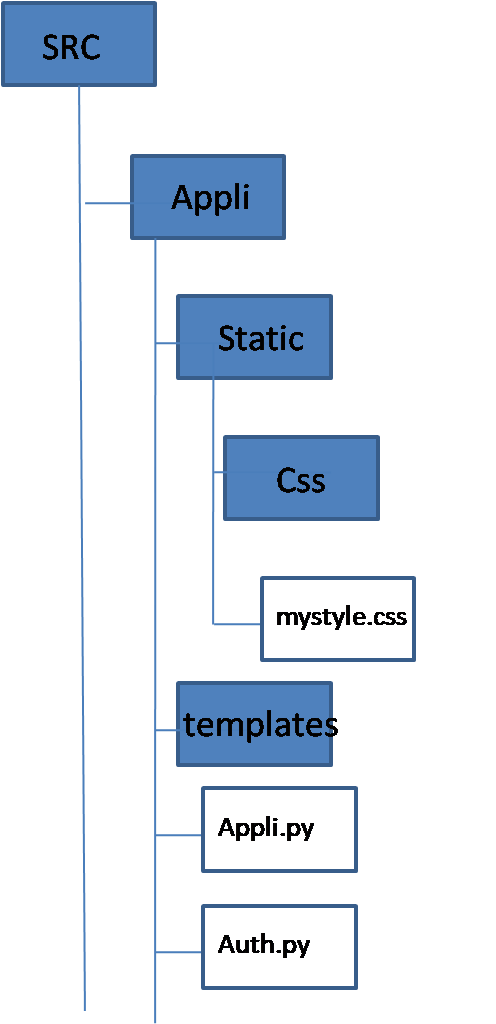
\includegraphics[width=5cm]{archifront.png}\\
         \textbf{Figure:}Architecture du Front-end
         \end{center}
 Les fichiers auth.py et appli.py qui instancient les formulaires contenant leur paramètre d'entrée ainsi que les templates HTML associés.
\subsubsection{Automatisation avec un script SH}
\textbf{launchapp.sh} permet de lancer l'application dans l'environnement virtuel de manière simplifiée afin de maximiser l'expérience de l'utilisateur.
 \subsection{Interface Graphique Générale}
 Il tient à préciser que le design graphique de notre application a pour inspiration le site officiel de l'Institut Mines-Télécom. La bar de navigation est commune à toutes les pages du sites et possèdent un bouton download qui à l'aide de URL obtenue par une fonction Javascript (request.url)
 \subsubsection{Bulma et Css}
 Pour le design de notre site Web, nous avons choisi le Flat Design plutôt que le Skeuomorphisme, qui permet de supprimer toutes les informations non-essentielles à l'utilisateur. Le choix de Bulma s'est donc imposé comme une évidence non seulement grâce à son utilisation pratique mais aussi grâce au design de ses assets, connus pour son flat design. Ainsi nous avons adapté à nos besoins les divers assets du sites ainsi pris pour inspiration en plus du color scheme et de la forme triangulaire. 
  \begin{center}
         
\includegraphics[width=3cm]{favicon.png}\\
         \textbf{Figure:}Icône de l'IMT modifiée pour signifier la notification 
         \end{center}
 De la même manière, nous avons implémenté un carrousel pour la page d'accueil à partir du fichier  mystyle.css dans lequel  sont implémentés un At-Rules keyframes modifiés ainsi qu'un At-Rules media adapté.

 \section{Partie Back-end de l'application}
 Il s'agit principalement des fonctions de création de base de données que l'on a présenté dans le chapitre précédent ainsi que l'installation de l'ensemble des dépendances de l'application. Nous avons également crée un script SH config.sh pour installer et configurer l'environnement du Back-end.
 \subsection{Architecture du Back-end}
 L'architecture est donc détaillée dans la figure suivante de manière simplifiée:
   \begin{center}
         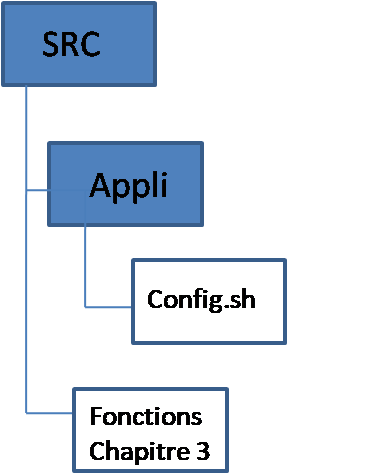
\includegraphics[width=5cm]{backendarch.png}\\
         \textbf{Figure:}Architecture du Back-end
         \end{center}\\
    Le Back-end utilise alors le principe de microservices, c'est à dire qu'ils utilisent plein de petits services différents plutôt qu'un code monolithique. Il y a plusieurs avantages à utiliser des microservices: mais celle qui ressort le plus c'est l'indépendance.En effet ces différents services sont testés et utilisés de façon indépendantes.
    
      \begin{center}
         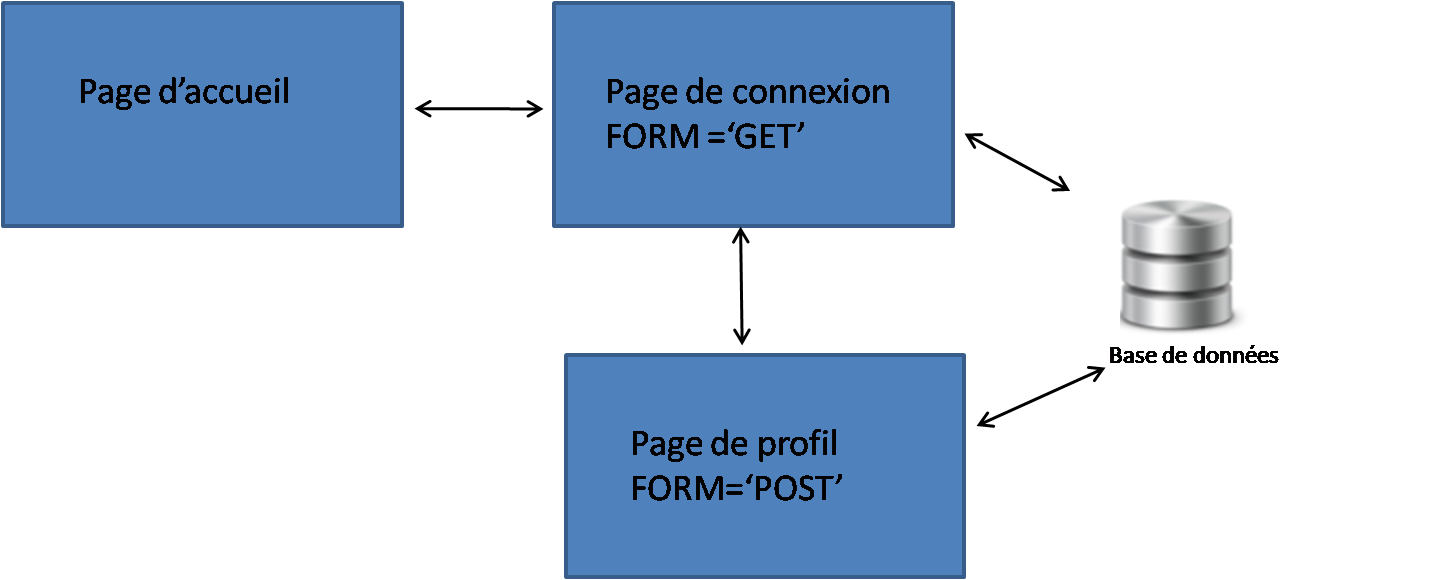
\includegraphics[width=15cm]{schsite.png}\\
         \textbf{Figure:}Architecture du site
         \end{center}\\